\documentclass[12pt,a4paper]{report}

\usepackage[portuguese]{babel}
\usepackage{hyphenat}
\usepackage{amsmath}
\usepackage{amsfonts}
\usepackage{amssymb}
\usepackage{amsthm}
\usepackage{graphicx}
\usepackage{makeidx}
\usepackage{enumerate}
\usepackage[square,sort,comma,numbers]{natbib}
\usepackage[left=1.25in,right=1in,top=1in,bottom=1in]{geometry}
\usepackage{setspace}

\setstretch{1.5}

\hyphenpenalty
\exhyphenpenalty

\begin{document}

\begin{titlepage}
    {\centering
        {
        \LARGE{\textbf{Projeto Laboratórios de Informática III\\Fase 1}} \\ 
        \vspace*{\fill} 
        {\large{Projeto desenvolvido por}} \\
        \vspace 
        \large{ Fábio  Leite (A100902),  Luís Figueiredo (A100549) e Gonçalo Gonçalves (A100833)} \\
        {\small{Grupo 50}}
        \vspace*{\fill} \\
        {\Large Licenciatura em Engenharia Informática} \\
        \vspace*{\fill}
        
\includegraphics[scale=1.25]{eeng.png} \\ [0.5cm]
        {\large Departamento de Informática \\ Universidade do Minho} \\
        }
    }
\end{titlepage}

\newpage

    \tableofcontents

\newpage

    \chapter{Introdução}
    Este projeto está a ser desenvolvido no âmbito da unidade curricular de Laboratórios de Informática III do ano 2023/2024. Neste projeto é nos instruída a implementação de uma base de dados em memória que armazene dados fornecidos em ficheiros ".csv". \\
    O projeto está dividido em duas fases, e esta primeira fase consiste em implementar o \textit{parsing} dos dados e em executar várias \textit{queries} sobre os dados, estando esses pedidos armazenados num ficheiro de texto cujo caminho é recebido como argumento. \\
      Para a execução deste projeto foi usada a biblioteca \textit{glib} uma vez que esta biblioteca possui implementações de várias estruturas úteis. 
 
\newpage
	
    \chapter{Desenvolvimento}


    No desenvolvimento da aplicação começamos por imaginar uma arquitetura que representaria a ligação entre os diferentes ficheiros que iriam compor o programa e a forma como iriam comunicar entre si, tentando garantir a existência  do encapsulamento e modularidade durante o desenvolvimento do projeto. Após alguma discussão sobre a estrutura que iriamos adotar, chegamos ao seguinte modelo: 
    
    \begin{figure}[h]
    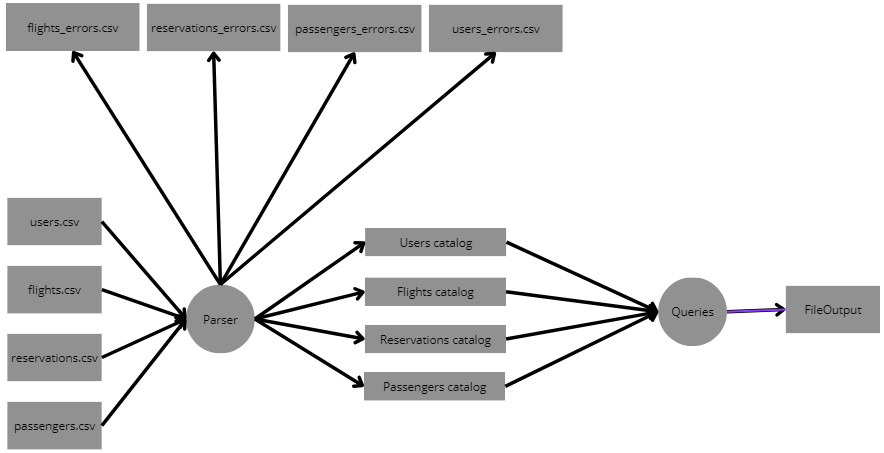
\includegraphics[scale = 0.5]{diagrama.png}
    \centering
    \caption{Diagrama da estrutura utilizada para o projeto}
    \end{figure} 

    
    O passo inicial foi perceber como devíamos armazenar os dados. Optamos por usar \textit{hashtables} para os ficheiros que apresentavam mais dados \textit{(users.csv,flights.csv, reservations.csv)} devido ao facto de estas oferecerem um tempo de pesquisa constante. Reparámos que o \textit{passengers.csv} apresenta apenas dois elementos: user\_id e flight\_id. Estes id's podem ser repetidos ao longo do ficheiro e, portanto, não faria sentido usar nenhum deles como \textit{key} de uma \textit{hashtable}. Foi decidido, então, guardar os dados deste ficheiro numa lista ligada (GList). 
    Já na parte prática, (tendo sempre a modularidade em conta) criámos \textit{structs} para guardar cada linha do ficheiro, dividindo os diferentes campos da mesma nos respetivos atributos. Depois implementámos os catálogos de modo a armazenarem várias destas \textit{structs} (PASSENGER, FLIGHT, USER e RESERVATION).  

    Críamos o \textit{Parser} que é responsável por tratar os ficheiros .csv na pasta cujo caminho é fornecido como 1º argumento ao executar o programa e, posteriormente, encaminhar os dados para as respetivas estruturas onde a informação vai ser guardada. O \textit{parser} chama funções do módulo \textit{Validation} ao fazer o seu trabalho de modo a garantir a validação dos dados armazenados. Em caso de erro, envia-os para o módulo \textit{Output} que escreve nos ficheiros de erros correspondentes todas as linhas do ficheiro original que continham qualquer erro.

    Depois disto, implementámos o módulo \textit{Interpreter} que é responsável por interpretar os comandos passados pelo ficheiro .txt de input passado como 2º argumento ao executar o programa, chamando a função correspondente implementada no módulo \textit{Queries}, onde é permitido o acesso aos catálogos para que o resultado da \textit{query} seja retornado (já devidamente formatado) ao \textit{Interpreter}, que, por sua vez, o envia para o \textit{Output} para que este possa escrevê-lo deviadamente em ficheiros commandX\_output.txt que, caso não existam, são criados.

    Isto tudo tendo em conta as regras de encapsulamento que, apesar de adicionar uma camada extra de complexidade ao código por ser mais difícil acessar e modificar certos dados, permitiram-nos desenvolver um sistema mais robusto e modular ao evitar acesso não autorizado e facilitando a manutenção do código a longo prazo.

    %TODO: ver o que por das queries 
    
    \begin{figure}[h]
    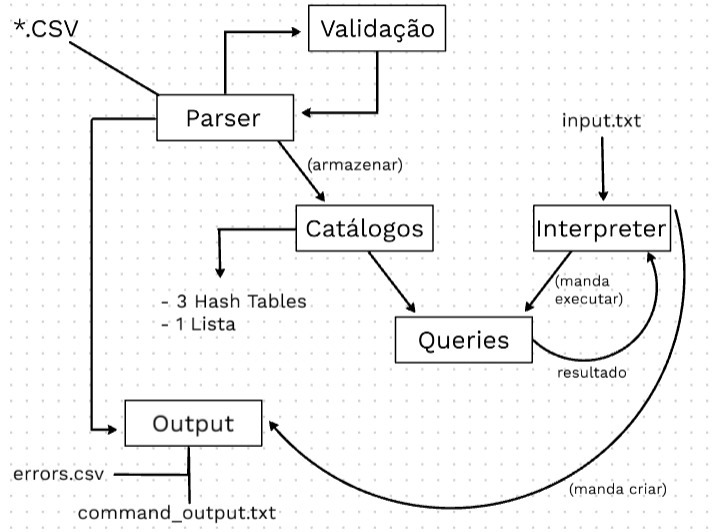
\includegraphics[scale = 0.7]{diagrama2.jpeg}
    \centering
    \caption{Diagrama do funcionamento do programa}
    \end{figure} 
    
\newpage

    \chapter{Dificuldades sentidas}

    \paragraph{} Ao longo do desenvolvimento do projeto, fomos encontrando diversos problemas que, para além de produzirem resultados errados, também impediram o nosso progresso.
    Primeiramente, sentimos uma grande dificuldade na validação de certos dados, sendo que alguns deles(na nossa prespetiva) só poderiam ser validados após a inserção dos mesmos nas nossas estruturas.
    \par Da mesma forma, certas queries levantaram-nos dúvidas, especialmente a query 9. Nesta query, a nossa dúvida principal é provocada pelo facto de a mesma provocar \textit{segmentation fault} na plantaforma de testes, embora a mesma não o faça localmente.
    \par Por fim, a utilização da \textit{glib}, embora traga bastantes benefícios,também traz uma maior complexidade para o projeto, sendo necessários vários momentos de pesquisa e teste para perceber as funcionalidades que as estruturas de dados e as funções desta mesma biblioteca apresentam.
    
   
    

\newpage

    \chapter{Conclusão}

    \paragraph{}Dado o problema proposto, no nosso ponto de vista, a resolução por nós implementada
cumpre grande parte dos principais objetivos desta primeira fase. 
Para o armazenamento da informação recolhida pelo parsing dos dados dos ficheiros .csv, foi
por nós usado hash tables por considerarmos o método mais eficiente e rápido na procura dos
dados para a resolução das queries propostas e uma lista ligada uma vez que a utilização de uma tabela de hash neste caso não seria justificada.
\par Embora apresentemos 6 queries no nosso projeto, algumas delas não se apresentam corretamente implementadas, sendo esse um dos principais pontos a melhorar para a próxima fase. Da mesma forma, também pretendemos melhorar a qualidade do código para próxima fase, uma vez que o consideramos um pouco confuso.

        
\end{document}
